
%(BEGIN_QUESTION)
% Copyright 2015, Tony R. Kuphaldt, released under the Creative Commons Attribution License (v 1.0)
% This means you may do almost anything with this work of mine, so long as you give me proper credit

\noindent
{\bf Lab Exercise -- introduction}

\vskip 5pt

Your team's task is to construct and test a safety ``shutdown'' system designed to bring some process to an idle condition if one or more variables drift beyond acceptable parameters.  This may take the form of an additional layer of sensors and controls incorporated into your existing process control loop (e.g. a high-pressure shutdown system on an air pressure control loop), or it may be entirely separate (e.g. a protective relay system designed to trip a circuit breaker on excessive load current).

If implemented as an additional layer of controls to a functioning process loop, the shutdown function must bring the process to a ``safe'' condition (power off, vessels drained/vented, etc.) independent of any action on the part of the loop PID controller.  In other words, the safety function must work {\it no matter what the loop controller is trying to do}.  This shutdown condition must ``latch'' and be re-settable only from a manual pushbutton, also independent of the loop PID controller.  You may use either a hard-wired relay, a PLC, or a dedicated safety controller to implement the latching safety shutdown function.  The safety control element \underbar{must be a solenoid valve} if the process final control element is pneumatically actuated!

The following table of objectives show what you and your team must complete within the scheduled time for this lab exercise.  Note how some of these objectives are individual, while others are for the team as a whole:

\underbar{Objective completion table:}

% No blank lines allowed between lines of an \halign structure!
% I use comments (%) instead, so that TeX doesn't choke.

$$\vbox{\offinterlineskip
\halign{\strut
\vrule \quad\hfil # \ \hfil & 
\vrule \quad\hfil # \ \hfil & 
\vrule \quad\hfil # \ \hfil & 
\vrule \quad\hfil # \ \hfil & 
\vrule \quad\hfil # \ \hfil & 
\vrule \quad\hfil # \ \hfil & 
\vrule \quad\hfil # \ \hfil \vrule \cr
\noalign{\hrule}
%
% First row
{\bf Performance objective} & {\bf Grading} & {\bf 1} & {\bf 2} & {\bf 3} & {\bf 4} & {\bf Team} \cr
%
\noalign{\hrule}
%
% Another row
Shutdown system design approval & mastery & -- & -- & -- & -- & \cr
%
\noalign{\hrule}
%
% Another row
Team meeting and prototype sketch & mastery & -- & -- & -- & -- & \cr
%
\noalign{\hrule}
%
% Another row
Final loop diagram and system inspection & mastery & & & & & -- -- -- -- \cr
%
\noalign{\hrule}
%
% Another row
Demonstration of working system & mastery & -- & -- & -- & -- & \cr
%
\noalign{\hrule}
%
% Another row
Safety ``trip'' testing (5 minute time limit) & mastery & & & & & -- -- -- -- \cr
%
\noalign{\hrule}
%
% Another row
Lab question: Instrument connections & proportional &  &  &  &  & -- -- -- -- \cr
%
\noalign{\hrule}
%
% Another row
Lab question: Commissioning & proportional &  &  &  &  & -- -- -- -- \cr
%
\noalign{\hrule}
%
% Another row
Lab question: Mental math & proportional &  &  &  &  & -- -- -- -- \cr
%
\noalign{\hrule}
%
% Another row
Lab question: Diagnostics & proportional &  &  &  &  & -- -- -- -- \cr
%
\noalign{\hrule}
%
% Another row
Decommission and lab clean-up & mastery & -- & -- & -- & -- &  \cr
%
\noalign{\hrule}
%
% Another row
Team tool locker inspection & mastery & -- & -- & -- & -- &  \cr
%
\noalign{\hrule}
} % End of \halign 
}$$ % End of \vbox

The only ``proportional'' scoring in this activity are the lab questions, which are answered by each student individually.  A listing of potential lab questions are shown at the end of this worksheet question.  The lab questions are intended to guide your labwork as much as they are intended to measure your comprehension, and as such the instructor may ask these questions of your team day by day, rather than all at once (on a single day).

\vskip 10pt

{\bf It is essential that your team plans ahead what to accomplish each day.  A short (10 minute) team meeting at the beginning of each lab session is a good way to do this, reviewing what's already been done, what's left to do, and what assessments you should be ready for.  There is a lot of work involved with building, documenting, and testing these working instrument systems!}

As you and your team work on this system, you will invariably encounter problems.  You should always attempt to solve these problems as a team before requesting instructor assistance.  If you still require instructor assistance, write your team's color on the lab whiteboard with a brief description of what you need help on.  The instructor will meet with each team in order they appear on the whiteboard to address these problems.




\vfil \eject

\noindent
{\bf Lab Exercise -- team meeting, prototype sketch, and instrument selection}

\vskip 5pt

An important first step in completing this lab exercise is to {\bf meet with your instructor} as a team to discuss safety concerns, team performance, and specific roles for team members.  If you would like to emphasize exposure to certain equipment (e.g. use a particular type of control system, certain power tools), techniques (e.g. fabrication), or tasks to improve your skill set, this is the time to make requests of your team so that your learning during this project will be maximized.

\vskip 10pt

An absolutely essential step in completing this lab exercise is to work together as a team to {\bf sketch a prototype diagram} showing what you intend to build.  This usually takes the form of a simple electrical schematic and/or loop diagram showing all electrical connections between components, as well as any tubing or piping for fluids.  This prototype sketch need not be exhaustive in detail, but it does need to show enough detail for the instructor to determine if all components will be correctly connected for their safe function.

For example, if you intend to connect field devices to a PLC (Programmable Logic Controller), your prototype sketch must show how those devices will connect to typical input/output terminals on the PLC, where electrical power will be supplied, etc.  Prototype sketches need not show all intermediary connections between components, such as terminal blocks in junction boxes between the field device and the controller.

You should practice good problem-solving techniques when creating your prototype sketch, such as consulting equipment manuals for information on component functions and marking directions of electric current, voltage polarities, and identifying electrical sources/loads.  Use this task as an opportunity to strengthen your analytical skills!  Remember that you will be challenged in this program to do all of this on your own (during ``capstone'' assessments), so do not make the mistake of relying on your teammates to figure this out for you -- instead, treat this as a problem {\it you} must solve and compare your results with those of your teammates.

Your team's prototype sketch is so important that the instructor will demand you provide this plan before any construction on your team's working system begins.  {\it Any team found constructing their system without a verified plan will be ordered to cease construction and not resume until a prototype plan has been drafted and approved!}  Similarly, you should not deviate from the prototype design without instructor approval, to ensure nothing will be done to harm equipment by way of incorrect connections.  Each member on the team should have ready access to this plan (ideally possessing their own copy of the plan) throughout the construction process.  Prototype design sketching is a skill and a habit you should cultivate in school and take with you in your new career.

\vskip 10pt

Your first design step needs to be deciding what process variable to monitor in your system, and what the automated shutdown action(s) should be.  The variable to monitor may or may not be the process variable (PV) being regulated by the loop controller.  Whatever action the shutdown system automatically takes, however, should completely override the action of the loop controller in a shutdown condition.

Once you have defined the shutdown variable and action(s), the next step is to design an independent control system to add to your working process.  This SIS (Safety Instrumented System) needs to be based on a {\it latch:} the SIS will ``trip'' whenever a shutdown condition is detected, and will not ``reset'' (even after the condition clears) until an operator manually presses a reset pushbutton.  A typical SIS for the scope of a lab project such as this usually consists of these components:

\begin{itemize}
\item{} Sensor for detecting shutdown condition (separate from PV sensor used in the PID control system)
\item{} Threshold detection relay (outputs a discrete signal to trip the latch)
\item{} Latching system (e.g. electromechanical relay, PLC, or dedicated SIS controller)
\item{} FCE override (e.g. solenoid valve forcing the control valve to its ``fail-safe'' position)
\end{itemize}

Your instructor will verify that your team's SIS design is practical.  Note that the SIS need not be complex: in fact, simpler is better here.  A system consisting of a process switch, and an ice-cube relay to latch on as well as energize or de-energize a ``dump'' solenoid when tripped, is sufficient for many student-built processes.  If your SIS sensor is a 4-20 mA analog transmitter, you will need some ``alarm'' module or relay to trigger the latch.  A PLC with an analog input works well for this purpose, as does a stand-alone alarm module such as the Moore Industries DDA or SPA units.

\vskip 10pt

If your team plans to build a protective relay system, you will need to first select a suitable relay to use.  Modern digital relays such as the SEL model 501 are highly recommended.  Due to the fact your electrical load won't be drawing much current, you will need to use a CT (current transformer) with multiple turns of wire run through its core in order to achieve a workable load:relay current ratio.  I rule of thumb here is to not wrap more than 4 turns of wire through the core of the small CT you will be given, in order to avoid saturation and inaccurate performance.

\vskip 10pt

{\bf Planning a functioning system should take no more than an hour if the team is working efficiently, and will save you hours of frustration (and possible component destruction!).}







\vfil \eject

\noindent
{\bf Lab Exercise -- building/modifying the system}

\vskip 5pt

After getting your prototype sketch approved by the instructor, you are cleared to begin building your system.  Instruments attach to 2-inch pipes using special brackets and U-bolts.  These brackets and U-bolts are located in the instrument storage area.  

You may install your SIS control hardware inside the nearest field junction box.  The installation should be neat and professional, like the rest of the control system.  Instruments should attach to 2-inch pipes using special brackets and U-bolts, located in the instrument storage area.  Liquid-tight flexible conduits should be used to route signal cable between the instrument(s) and the junction box.

Finally, your SIS needs to have a loop number, so all instruments may be properly labeled.  This loop number needs to be unique, not only from other SIS installations in the lab but also different from the instruments used for regulatory control in the process (i.e. the PID controller, transmitter, FCE).

\vskip 10pt

If your choice of shutdown systems is a protective relay and circuit breaker, there will be no 2-inch-pipe-mount devices such as pressure transmitters.  Neither will there be ISA-standard loop numbers, as protective relays are labeled according their specific function rather than according to the general process.  You may choose to set up such a system entirely inside an electrical enclosure, or perhaps between two different enclosures (e.g. one for the circuit breaker and load, the other for the relay).  An ``open'' design such as on an enclosure subpanel is also acceptable, so long as all electrical terminals are ``touch-safe'' (recessed) so as to present little shock hazard and the system is locked and tagged out when not in use.

\vskip 10pt

{\bf Common mistakes:}

\begin{itemize}
\item{} Neglecting to consult the manufacturer's documentation for field instruments (e.g. how to wire them, how to calibrate them).
\item{} Mounting the field instrument(s) in awkward positions, making it difficult to reach connection terminals or to remove covers when installed.
\item{} Failing to tug on each and every wire where it terminates to ensure a mechanically sound connection.
\item{} Students working on portions of the system in isolation, not sharing with their teammates what they did and how.  It is important that the whole team learns all aspects of their system!
\end{itemize}






\vfil \eject

\noindent
{\bf Lab Exercise -- documenting the system}

\vskip 5pt

Each student must sketch their own {\it loop diagram} for their team's SIS, following proper ISA conventions.  The diagram for this lab exercise should be an expansion on the original loop diagram for the PID-controlled process, showing the regulatory instruments and controller as well as the (new) SIS instruments and control system.  The rationale for showing both ``layers'' of control on the same diagram is so that it becomes clear how the SIS system overrides the regulatory system.

As usual the new loop diagram must be {\it comprehensive} and {\it detailed}, showing every wire connection, every cable, every terminal block, range points, etc.  The principle to keep in mind here is to make the loop diagram so complete and unambiguous that anyone can follow it to see what connects to what, even someone unfamiliar with industrial instrumentation.  In industry, loops are often constructed by contract personnel with limited understanding of how the system is supposed to function.  The loop diagrams they follow must be so complete that they will be able to connect everything properly without necessarily understanding how it is supposed to work.

Every instrument and every signal cable in your loop needs to be properly labeled with an ISA-standard tag number.  An easy way to do this is to wrap a short piece of masking tape around each cable (and placed on each instrument) then writing on that masking tape with a permanent marker.  Although no industry standard exists for labeling signal cables, a good recommendation is to label each two-wire cable with the tag number of the field instrument it goes to.  Thus, every length of two-wire cable in a pressure transmitter circuit should be labeled ``PT-$x$'' (where ``$x$'' is the loop number), every flow control valve should be labeled ``FV-$x$'', etc.  Remember that the entire loop is defined by the process variable it measures: if the PV is {\it temperature} then the transmitter with be a {\it T}T, the control valve will be a {\it T}V, the controller with be a {\it T}C, etc.

\vskip 10pt

Protective relay systems follow an entirely different schematic diagram convention from ISA loop diagrams.  Examples of such diagrams will likely be found in the manual of the protective relay you choose, as well as within the INST263 homework questions.  Just like loop diagrams, though, every wire connection, every cable, and every terminal block must be clearly documented.  It must be so complete and unambiguous that anyone can follow it regardless of specific experience with protective relays.

\vskip 10pt

When your entire team is finished drafting your individual diagrams, call the instructor to do an inspection of the loop.  Here, the instructor will have students take turns going through the entire loop, with the other students checking their diagrams for errors and omissions along the way.  During this time the instructor will also inspect the quality of the installation, identifying problems such as frayed wires, improperly crimped terminals, poor cable routing, missing labels, lack of wire duct covers, etc.  The team must correct all identified errors in order to receive credit for their system.  

After successfully passing the inspection, each team member needs to place their loop diagram in the diagram holder located in the middle of the lab behind the main control panel.  When it comes time to troubleshoot another team's system, this is where you will go to find a loop diagram for that system!

\vskip 10pt

{\bf Common mistakes:}

\begin{itemize}
\item{} Forgetting to label all signal wires (see example loop diagrams).
\item{} Forgetting to label all field instruments with their own tag names (e.g. PT-83).
\item{} Forgetting to note all wire colors.
\item{} Forgetting to put your name on the loop diagram!
\item{} Basing your diagram off of a team-mate's diagram, rather than closely inspecting the system for yourself.
\item{} Not placing loop sheet instruments in the correct orientation (field instruments on the left, control room instruments on the right).
\end{itemize}

\vskip 10pt

{\bf Creating and inspecting accurate loop diagrams should take no more than one full lab session (3 hours) if the team is working efficiently!}





\vfil \eject

\noindent
{\bf Lab Exercise -- safety ``trip'' testing}

\vskip 5pt

Instead of troubleshooting a fault in the system as is customary for lab exercises, your task in this lab is to test a SIS (Safety Instrumented System) to ensure its proper operation with the process fully operational, without actually ``tripping'' the control system and switching it into shut-down mode.  The goal is to validate the correct operation of as much of the SIS as possible without actually shutting down the process.  All ``trip'' testing is done on an individual basis (no team credit!), and must be done {\it on a system you did not help build}, so that you must rely on schematic diagrams to find your way around the system and to determine how to do the test instead of from your own memory of building it.

The instructor will choose the SIS for you to test.  This may be a process constructed by another student team, or it may be one of the permanently constructed processes in the lab (e.g. the turbocompressor system, the protective relay demonstration system, one of the protective relays in the lab's miniature AC power grid system).

There may very well be more than one acceptable way to perform a ``trip'' test.  The instructor will specify conditions to make your test slightly different from other tests performed on the same system.  For example, the instructor may ask you to {\it electrically} simulate a trip condition (e.g. use a loop calibrator to simulate a transmitter signal at the trip level), or may ask you to {\it physically} simulate the same trip condition (e.g. stimulate the SIS sensor with the proper amount of millivoltage, pressure, etc.), while you must determine how to bypass the controls so that a sensor trip signal does not actually initiate a shutdown.  The conditions of bypass may also be randomized.  For example, if the SIS actuating element is a pneumatic solenoid valve, the instructor may ask you to bypass the solenoid {\it electrically} to avoid an actual system shutdown (e.g. prevent the solenoid from being ``told'' to trip), or the instructor may ask you to bypass the solenoid {\it pneumatically} so that the solenoid will not shut down the system even when it is electrically tripped.

Each student is given a limited amount of time to plan their test after having been given the conditions by the instructor.  The test must then begin by the end of this time period -- and the test must successfully show the SIS system to be working without an actual shutdown occurring -- for credit.  All testing activities will take place under direct instructor supervision to ensure students are working independently and efficiently. 

Failure to formulate a test strategy at the end of the allotted time, failure to conclusively demonstrate that the SIS system is functioning as designed, or actually shutting down the system will disqualify the effort, in which case the student must re-try with a different set of conditions (perhaps on a different system as well).  Multiple re-tries are permitted with no reduction in grade.

A standard multimeter and signal source (e.g. loop calibrator or protective relay test set) are the only pieces of test equipment allowed during the time limit.

\vskip 10pt

{\bf Common mistakes:}

\begin{itemize}
\item{} Making or breaking electrical connections in such a way that causes the system to trip before the test is supposed to begin
\item{} Neglecting to confirm the system's status with a multimeter before proceeding
\item{} Incorrectly interpreting the loop diagram (e.g. thinking you're at the wrong place in the system when taking measurements).
\item{} Incorrect multimeter usage (e.g. AC rather than DC, wrong range, wrong test lead placement).  This is especially true when a student comes to lab unprepared and must borrow someone else's meter that is different from theirs!
\end{itemize}

\vskip 10pt

{\bf Even though this exercise is not called ``troubleshooting,'' it is every bit as analytical as system diagnosis, and may require some amount of creativity to pull off.  This takes a lot of lab time, usually at least two 3-hour lab sessions for everyone in a full class to successfully pass.  Be sure your team budgets for this amount of time as you plan your work, and also be sure to take advantage of your freedom to observe others as they trip-test, to better learn this art.}









\vfil \eject

\noindent
{\bf Lab questions}

\vskip 5pt

\begin{itemize}
\item{} {\bf Instrument connections}
\item{} Determine correct wire connections between instruments to create a working 4-20 mA loop circuit, based on diagrams of instruments with terminals labeled
\item{} Correctly determine all electrical sources and loads, as well as all voltage polarities and current directions in a 4-20 mA loop circuit, based on diagrams of instruments with terminals labeled
\end{itemize}

\filbreak

\begin{itemize}
\item{} {\bf Commissioning and Documentation}
\item{} Explain what ``1oo1'' means when defined in terms of {\it dependability} versus when it is defined in terms of {\it security} 
\item{} Explain what ``1oo2'' means when defined in terms of {\it dependability} versus when it is defined in terms of {\it security} 
\item{} Explain what ``2oo2'' means when defined in terms of {\it dependability} versus when it is defined in terms of {\it security} 
\item{} Explain what ``2oo3'' means when defined in terms of {\it dependability} versus when it is defined in terms of {\it security} 
\item{} Explain how the ``latch'' portion of your team's SIS functions
\item{} Explain what ``deadband'' means in reference to the trip threshold of your system's SIS sensor or relay
\item{} Explain proper three-valve manifold operating procedures (for both placing in and taking out of service)
\end{itemize}

\filbreak

\begin{itemize}
\item{} {\bf Mental math} (no calculator allowed!)
\item{} Calculate the dependability of a ``1oo2 trip'' system given the probabilities of unresponsive (``dangerous'') failures for each element, also explaining the rationale for your calculation
\item{} Calculate the dependability of a ``2oo2 trip'' system given the probabilities of unresponsive (``dangerous'') failures for each element, also explaining the rationale for your calculation
\item{} Calculate the security of a ``1oo2 trip'' system given the probabilities of false-alarm (``safe'' failures) for each element, also explaining the rationale for your calculation
\item{} Calculate the security of a ``2oo2 trip'' system given the probabilities of false-alarm (``safe'' failures) for each element, also explaining the rationale for your calculation
\end{itemize}

\filbreak

\begin{itemize}
\item{} {\bf Diagnostics}
\item{} Explain how to distinguish an ``open'' cable fault from a ``shorted'' cable fault using only a voltmeter (no current or resistance measurement, but assuming you are able to break the circuit to perform the test)
\item{} Identify how to electrically simulate a shutdown trip condition (i.e. without actually having to stimulate the sensor itself)
\item{} Identify how to test the proper operation of the shutdown sensor without actually shutting the system down
\item{} Determine whether or not a given diagnostic test will provide useful information, given a set of symptoms exhibited by a failed system
\item{} Identify at least two plausible faults given the results of a diagnostic test and a set of symptoms exhibited by a failed system
\item{} Propose a diagnostic test for troubleshooting a failed system and then explain the meanings of two different test results
\end{itemize}



\vfil \eject

\noindent
{\bf Lab Exercise -- decommissioning and clean-up}

\vskip 5pt

The final step of this lab exercise is to decommission your team's entire system and re-stock certain components back to their proper storage locations, the purpose of which being to prepare the lab for the next lab exercise.  Remove your system documentation (e.g. loop diagram) from the common holding area, either discarding it or keeping it for your own records.  Also, remove instrument tag labels (e.g. FT-101) from instruments and from cables.  Perform general clean-up of your lab space, disposing of all trash, placing all tools back in their proper storage locations, sweeping up bits of wire off the floor and out of junction boxes, etc.

\vskip 10pt

\indent
{\bf Leave the following components in place, mounted on the racks:}

\begin{itemize}
\item{} Large control valves and positioners
\item{} I/P transducers
\item{} Large electric motors
\item{} Large variable-frequency drive (VFD) units
\item{} Cables inside conduit interconnecting junction boxes together
\item{} Pipe and tube fittings (do not unscrew pipe threads)
\item{} Supply air pressure regulators
\end{itemize}

\vskip 10pt

\indent
{\bf Return the following components to their proper storage locations:}

\begin{itemize}
\item{} Sensing elements (e.g. thermocouples, pH probes, etc.)
\item{} Process transmitters
\item{} ``Jumper'' cables used to connect terminal blocks within a single junction box
\item{} Plastic tubing and tube fittings (disconnect compression-style tube fittings)
\item{} Power cables and extension cords
\item{} Adjustment (loading station) air pressure regulators
\end{itemize}

\vskip 10pt

Finally, you shall return any control system components to their original (factory default) configurations.  This includes controller PID settings, function block programs, input signal ranges, etc.


\underbar{file i02406}
%(END_QUESTION)





%(BEGIN_ANSWER)


%(END_ANSWER)





%(BEGIN_NOTES)

\noindent
{\bf Loop diagrams / inspections:}

I strongly recommend checking off students' loop diagrams while you inspect their loop (checking for secure wiring, proper tubing, good conduit installation, etc.) with them.  Have all team members take you on a ``tour'' of their completed loop, with each team member explaining a different portion of the loop you select while using their own loop diagram as a guide.  While a student is explaining their section of the loop, you can check the other students' loop diagrams for accuracy.  This not only saves time by consolidating the tasks of loop inspection and loop diagram verification, but it also ensures students can actually relate their loop diagrams to the loop they have built and articulate that understanding to you.

\vskip 10pt

\goodbreak

\noindent
{\bf Safety Trip Testing scenarios:}

\begin{itemize}
\item{} {\bf Turbocompressor system:}
\item{} Test the operation of the low oil pressure switch contacts, without activating the PLC shutdown logic
\item{} Test the operation of the low oil level switch contacts, without activating the PLC shutdown logic
\item{} Test the operation of the pump vibration detector output (the Bently-Nevada vibration monitor), without activating the PLC shutdown logic
\item{} Test the operation of the high air temperature switch contacts (part of the Bently-Nevada monitor), without activating the PLC shutdown logic
\item{} Test the operation of the high oil temperature switch contacts (part of the Bently-Nevada monitor), without activating the PLC shutdown logic
\item{} Test the operation of the Emergency Stop pushbutton switch contacts, without activating the PLC shutdown logic
\item{} Activate the PLC shutdown logic by mechanically simulating a low oil pressure condition, without actually shutting the turbocompressor down
\item{} Activate the PLC shutdown logic by electrically simulating a low oil pressure condition to the PLC, without actually shutting the turbocompressor down
\item{} Activate the PLC shutdown logic by simulating a high air temperature condition using a thermocouple simulator, without actually shutting the turbocompressor down
\item{} Activate the PLC shutdown logic by simulating a high oil temperature condition using a thermocouple simulator, without actually shutting the turbocompressor down
\item{} Activate the PLC shutdown logic by pressing the Emergency Stop pushbutton, without actually shutting the turbocompressor down
\item{} Shut down the turbocompressor by mechanically simulating a low oil pressure condition
\item{} Shut down the turbocompressor by electrically simulating a low oil pressure condition to the PLC
\item{} Shut down the turbocompressor by mechanically simulating a low oil level condition
\item{} Shut down the turbocompressor by electrically simulating a high pump shaft vibration condition to the PLC
\item{} Shut down the turbocompressor by electrically simulating a high air temperature condition to the PLC
\item{} Shut down the turbocompressor by electrically simulating a high oil temperature condition to the PLC
\end{itemize}

\vskip 10pt

\filbreak

\begin{itemize}
\item{} {\bf Overcurrent protective relay system:}
\item{} Test the protective relay by simulating a time-overcurrent condition (with either a maximum or minimum trip time based on the relay's curve) on a specific phase, without actually tripping the circuit breaker
\item{} Test the protective relay by simulating a time-overcurrent condition (with either a maximum or minimum trip time based on the relay's curve) on a specific phase, allowing the circuit breaker to trip
\item{} Change the relay's time-overcurrent pickup value to a specified value and set the time dial such that the relay will trip in a specified amount of time at $x \times$ pickup, and then simulate that condition on a specific phase, allowing the circuit breaker to trip
\item{} Test the protective relay by simulating an instantaneous overcurrent condition on a specific phase, without actually tripping the circuit breaker
\item{} Test the protective relay by simulating an instantaneous overcurrent condition on a specific phase, allowing the circuit breaker to trip
\item{} Change the relay's instantaneous overcurrent pickup value to a specified value, and then simulate that condition on a specific phase, allowing the circuit breaker to trip
\item{} Manually assert a trip output command through the protective relay's front panel controls, without actually tripping the circuit breaker
\end{itemize}












\vfil \eject

\noindent
{\bf Lab questions}

\vskip 20pt

\item{$(1)$} Sketch correct wire connections between these instruments to create a working pressure measurement system, where both the single-loop controller and the DAQ unit register pressure sensed by the transmitter.  Feel free to use any appropriate channel on the DAQ unit:

$$\includegraphics[width=15.5cm]{i02406x01.eps}$$

\vskip 20pt

\item{$(2)$} Explain what {\it 2oo2 dependability} means for a set of redundant safety valves, designed to shut off process fluid flow in order to bring that process to a safe condition.

\vskip 20pt

\item{$(3)$} Suppose a set of redundant sensors is {\it 1oo2 to trip}, which means either one of the two sensors sensing a dangerous condition is sufficient to initiate a ``trip'' event and thereby bring the process to a shutdown (safe) condition.  If each of these two sensors has a 0.002 probability of failing in a dangerous state (i.e. being unresponsive when faced with a dangerous process condition), calculate the {\it dependabilty} of the redundant sensor set as a whole.

\vskip 20pt

\item{$(4)$} During typical operation, this SIS logic solver has the following I/O statuses: IN1 = energized ; IN2 = energized ; IN3 = de-energized ; IN4 = energized ; OUT1 = energized ; OUT2 = de-energized.  Devise a way to {\it electrically simulate a high-temperature condition} in order to test whether the logic solver trips the shutdown valve as it should:

$$\includegraphics[width=15.5cm]{i02406x03.eps}$$ 
















\vfil \eject

\noindent
{\bf Lab questions}

\vskip 20pt

\item{$(1)$} Sketch correct wire connections between these instruments to create a working pressure measurement system, where both the single-loop controller and the DAQ unit register pressure sensed by the transmitter.  Feel free to use any appropriate channel on the DAQ unit:

$$\includegraphics[width=15.5cm]{i02406x02.eps}$$

\vskip 20pt

\item{$(2)$} Explain what {\it 1oo2 security} means for a set of redundant safety valves, designed to shut off process fluid flow in order to bring that process to a safe condition.

\vskip 20pt

\item{$(3)$} Suppose a set of redundant sensors is {\it 1oo2 to trip}, which means either one of the two sensors sensing a dangerous condition is sufficient to initiate a ``trip'' event and thereby bring the process to a shutdown (safe) condition.  If each of these two sensors has a 0.003 probability of alarming falsely (i.e. reporting a dangerous process condition when none exists), calculate the {\it security} of the redundant sensor set as a whole.

\vskip 20pt

\item{$(4)$} During typical operation, this SIS logic solver has the following I/O statuses: IN1 = energized ; IN2 = energized ; IN3 = de-energized ; IN4 = energized ; OUT1 = energized ; OUT2 = de-energized.  Devise a way to {\it electrically simulate a low-flow condition} in order to test whether the logic solver trips the shutdown valve as it should:

$$\includegraphics[width=15.5cm]{i02406x03.eps}$$ 


%$$\includegraphics[width=15.5cm]{i0016rx01.eps}$$ 


%INDEX% Lab exercise, safety shutdown (SIS) control

%(END_NOTES)


